% Options for packages loaded elsewhere
\PassOptionsToPackage{unicode}{hyperref}
\PassOptionsToPackage{hyphens}{url}
\PassOptionsToPackage{dvipsnames,svgnames,x11names}{xcolor}
%
\documentclass[
  letterpaper,
  DIV=11,
  numbers=noendperiod,
  oneside]{scrartcl}

\usepackage{amsmath,amssymb}
\usepackage{lmodern}
\usepackage{iftex}
\ifPDFTeX
  \usepackage[T1]{fontenc}
  \usepackage[utf8]{inputenc}
  \usepackage{textcomp} % provide euro and other symbols
\else % if luatex or xetex
  \usepackage{unicode-math}
  \defaultfontfeatures{Scale=MatchLowercase}
  \defaultfontfeatures[\rmfamily]{Ligatures=TeX,Scale=1}
\fi
% Use upquote if available, for straight quotes in verbatim environments
\IfFileExists{upquote.sty}{\usepackage{upquote}}{}
\IfFileExists{microtype.sty}{% use microtype if available
  \usepackage[]{microtype}
  \UseMicrotypeSet[protrusion]{basicmath} % disable protrusion for tt fonts
}{}
\makeatletter
\@ifundefined{KOMAClassName}{% if non-KOMA class
  \IfFileExists{parskip.sty}{%
    \usepackage{parskip}
  }{% else
    \setlength{\parindent}{0pt}
    \setlength{\parskip}{6pt plus 2pt minus 1pt}}
}{% if KOMA class
  \KOMAoptions{parskip=half}}
\makeatother
\usepackage{xcolor}
\usepackage[left=1in,marginparwidth=2.0666666666667in,textwidth=4.1333333333333in,marginparsep=0.3in]{geometry}
\setlength{\emergencystretch}{3em} % prevent overfull lines
\setcounter{secnumdepth}{-\maxdimen} % remove section numbering
% Make \paragraph and \subparagraph free-standing
\ifx\paragraph\undefined\else
  \let\oldparagraph\paragraph
  \renewcommand{\paragraph}[1]{\oldparagraph{#1}\mbox{}}
\fi
\ifx\subparagraph\undefined\else
  \let\oldsubparagraph\subparagraph
  \renewcommand{\subparagraph}[1]{\oldsubparagraph{#1}\mbox{}}
\fi


\providecommand{\tightlist}{%
  \setlength{\itemsep}{0pt}\setlength{\parskip}{0pt}}\usepackage{longtable,booktabs,array}
\usepackage{calc} % for calculating minipage widths
% Correct order of tables after \paragraph or \subparagraph
\usepackage{etoolbox}
\makeatletter
\patchcmd\longtable{\par}{\if@noskipsec\mbox{}\fi\par}{}{}
\makeatother
% Allow footnotes in longtable head/foot
\IfFileExists{footnotehyper.sty}{\usepackage{footnotehyper}}{\usepackage{footnote}}
\makesavenoteenv{longtable}
\usepackage{graphicx}
\makeatletter
\def\maxwidth{\ifdim\Gin@nat@width>\linewidth\linewidth\else\Gin@nat@width\fi}
\def\maxheight{\ifdim\Gin@nat@height>\textheight\textheight\else\Gin@nat@height\fi}
\makeatother
% Scale images if necessary, so that they will not overflow the page
% margins by default, and it is still possible to overwrite the defaults
% using explicit options in \includegraphics[width, height, ...]{}
\setkeys{Gin}{width=\maxwidth,height=\maxheight,keepaspectratio}
% Set default figure placement to htbp
\makeatletter
\def\fps@figure{htbp}
\makeatother
\newlength{\cslhangindent}
\setlength{\cslhangindent}{1.5em}
\newlength{\csllabelwidth}
\setlength{\csllabelwidth}{3em}
\newlength{\cslentryspacingunit} % times entry-spacing
\setlength{\cslentryspacingunit}{\parskip}
\newenvironment{CSLReferences}[2] % #1 hanging-ident, #2 entry spacing
 {% don't indent paragraphs
  \setlength{\parindent}{0pt}
  % turn on hanging indent if param 1 is 1
  \ifodd #1
  \let\oldpar\par
  \def\par{\hangindent=\cslhangindent\oldpar}
  \fi
  % set entry spacing
  \setlength{\parskip}{#2\cslentryspacingunit}
 }%
 {}
\usepackage{calc}
\newcommand{\CSLBlock}[1]{#1\hfill\break}
\newcommand{\CSLLeftMargin}[1]{\parbox[t]{\csllabelwidth}{#1}}
\newcommand{\CSLRightInline}[1]{\parbox[t]{\linewidth - \csllabelwidth}{#1}\break}
\newcommand{\CSLIndent}[1]{\hspace{\cslhangindent}#1}

\KOMAoption{captions}{tableheading}
\makeatletter
\makeatother
\makeatletter
\makeatother
\makeatletter
\@ifpackageloaded{caption}{}{\usepackage{caption}}
\AtBeginDocument{%
\ifdefined\contentsname
  \renewcommand*\contentsname{Table of contents}
\else
  \newcommand\contentsname{Table of contents}
\fi
\ifdefined\listfigurename
  \renewcommand*\listfigurename{List of Figures}
\else
  \newcommand\listfigurename{List of Figures}
\fi
\ifdefined\listtablename
  \renewcommand*\listtablename{List of Tables}
\else
  \newcommand\listtablename{List of Tables}
\fi
\ifdefined\figurename
  \renewcommand*\figurename{Figure}
\else
  \newcommand\figurename{Figure}
\fi
\ifdefined\tablename
  \renewcommand*\tablename{Table}
\else
  \newcommand\tablename{Table}
\fi
}
\@ifpackageloaded{float}{}{\usepackage{float}}
\floatstyle{ruled}
\@ifundefined{c@chapter}{\newfloat{codelisting}{h}{lop}}{\newfloat{codelisting}{h}{lop}[chapter]}
\floatname{codelisting}{Listing}
\newcommand*\listoflistings{\listof{codelisting}{List of Listings}}
\makeatother
\makeatletter
\@ifpackageloaded{caption}{}{\usepackage{caption}}
\@ifpackageloaded{subcaption}{}{\usepackage{subcaption}}
\makeatother
\makeatletter
\@ifpackageloaded{tcolorbox}{}{\usepackage[many]{tcolorbox}}
\makeatother
\makeatletter
\@ifundefined{shadecolor}{\definecolor{shadecolor}{rgb}{.97, .97, .97}}
\makeatother
\makeatletter
\@ifpackageloaded{sidenotes}{}{\usepackage{sidenotes}}
\@ifpackageloaded{marginnote}{}{\usepackage{marginnote}}
\makeatother
\makeatletter
\makeatother
\ifLuaTeX
  \usepackage{selnolig}  % disable illegal ligatures
\fi
\IfFileExists{bookmark.sty}{\usepackage{bookmark}}{\usepackage{hyperref}}
\IfFileExists{xurl.sty}{\usepackage{xurl}}{} % add URL line breaks if available
\urlstyle{same} % disable monospaced font for URLs
\hypersetup{
  pdftitle={Spectral relaxations of persistent rank invariants},
  pdfauthor={Matt Piekenbrock\textbackslash mathrm\{\}\^{}\textbackslash dagger \& Jose Perea\textbackslash mathrm\{\}\^{}\textbackslash ddagger},
  colorlinks=true,
  linkcolor={blue},
  filecolor={Maroon},
  citecolor={Blue},
  urlcolor={Blue},
  pdfcreator={LaTeX via pandoc}}

\title{Spectral relaxations of persistent rank invariants}
\usepackage{etoolbox}
\makeatletter
\providecommand{\subtitle}[1]{% add subtitle to \maketitle
  \apptocmd{\@title}{\par {\large #1 \par}}{}{}
}
\makeatother
\subtitle{With a focus on \emph{parameterized} settings}
\author{Matt Piekenbrock\(\mathrm{}^\dagger\) \& Jose
Perea\(\mathrm{}^\ddagger\)}
\date{}

\begin{document}
\maketitle
\ifdefined\Shaded\renewenvironment{Shaded}{\begin{tcolorbox}[sharp corners, breakable, interior hidden, boxrule=0pt, enhanced, borderline west={3pt}{0pt}{shadecolor}, frame hidden]}{\end{tcolorbox}}\fi

\hypertarget{vectorizing-diagrams}{%
\subsection{Vectorizing diagrams}\label{vectorizing-diagrams}}

There are many mappings from \(\mathrm{dgm}\)'s to function spaces
(e.g.~Hilbert spaces)

\begin{itemize}
\tightlist
\item
  Persistence Landscapes (Bubenik 2020)
\end{itemize}

\begin{figure}

{\centering \includegraphics[width=0.4\textwidth,height=\textheight]{pers_landscape_def.png}

}

\end{figure}

\[ \lambda(k, t) = \sup \{ h \geq 0 \mid \mathrm{rank}(H_p^{i-h} \to H_p^{i+h}) \geq k \} \]

\hypertarget{vectorizing-diagrams-1}{%
\subsection{Vectorizing diagrams}\label{vectorizing-diagrams-1}}

There are many mappings from \(\mathrm{dgm}\)'s to function spaces
(e.g.~Hilbert spaces)

\begin{itemize}
\tightlist
\item
  Persistence Landscapes (Bubenik 2020) + Learning applications (Kim et
  al. 2020)
\end{itemize}

\begin{figure}

{\centering \includegraphics[width=0.4\textwidth,height=\textheight]{pers_landscape_app.png}

}

\end{figure}

\[ \lambda(k, t) = \sup \{ h \geq 0 \mid \mathrm{rank}(H_p^{i-h} \to H_p^{i+h}) \geq k \} \]

\hypertarget{vectorizing-diagrams-2}{%
\subsection{Vectorizing diagrams}\label{vectorizing-diagrams-2}}

There are many mappings from \(\mathrm{dgm}\)'s to function spaces
(e.g.~Hilbert spaces)

Persistence Landscapes (Bubenik 2020) + Learning applications (Kim et
al. 2020)

Persistence Images (Adams et al. 2017)

\begin{figure}

{\centering \includegraphics[width=\textwidth,height=0.5\textheight]{pers_image_def.png}

}

\end{figure}

\[ \rho(f, \phi) = \sum\limits_{(i,j) \in \mathrm{dgm}} f(i,j) \phi(\lvert j - i \rvert)\]

\hypertarget{vectorizing-diagrams-3}{%
\subsection{Vectorizing diagrams}\label{vectorizing-diagrams-3}}

There are many mappings from \(\mathrm{dgm}\)'s to function spaces
(e.g.~Hilbert spaces)

Persistence Landscapes (Bubenik 2020) + Learning applications (Kim et
al. 2020)

Persistence Images (Adams et al. 2017) + Learning applications (Som et
al. 2020)

\begin{figure}

{\centering \includegraphics[width=\textwidth,height=0.5\textheight]{pers_image_app.png}

}

\end{figure}

\[ \rho(f, \phi) = \sum\limits_{(i,j) \in \mathrm{dgm}} f(i,j) \phi(\lvert j - i \rvert)\]

\hypertarget{vectorizing-diagrams-4}{%
\subsection{Vectorizing diagrams}\label{vectorizing-diagrams-4}}

There are many mappings from \(\mathrm{dgm}\)'s to function spaces
(e.g.~Hilbert spaces)

Persistence Landscapes (Bubenik 2020) + Learning applications (Kim et
al. 2020)

Persistence Images (Adams et al. 2017) + Learning applications (Som et
al. 2020)

A few others\ldots{}\(^1\)

\begin{figure}

{\centering \includegraphics[width=0.8\textwidth,height=1\textheight]{vec1.png}

}

\end{figure}

\marginnote{\begin{footnotesize}

See (Bubenik 2020) for an overview.

\end{footnotesize}}

\hypertarget{we-have-many-goals-in-common}{%
\subsection{We have many goals in
common\ldots{}}\label{we-have-many-goals-in-common}}

\begin{itemize}
\tightlist
\item
  Vectorize persistence information
\end{itemize}

\begin{itemize}
\tightlist
\item
  Optimize persistence invariants
\end{itemize}

\begin{itemize}
\tightlist
\item
  Leverage the stability of persistence
\end{itemize}

\begin{itemize}
\tightlist
\item
  Connect to other areas of mathematics
\end{itemize}

\includegraphics[width=3.125in,height=3.125in]{pers_image.png}

\includegraphics[width=3.125in,height=3.125in]{pers_landscape_app.png}

\includegraphics[width=4.16667in,height=3.125in]{stability.gif}

\includegraphics[width=2.60417in,height=2.60417in]{lsst.png}

\textbf{Can we achieve them without computing diagrams?\(^\ast\)}

\marginnote{\begin{footnotesize}

Image from: https://epfl-lts2.github.io/gspbox-html/doc/graphs/

\end{footnotesize}}

\hypertarget{this-talk}{%
\subsection{This Talk}\label{this-talk}}

In this talk we introduce a { \emph{spectral-relaxation} } of the rank
invariant that:

\begin{enumerate}
\def\labelenumi{\arabic{enumi}.}
\tightlist
\item
  Continuously interpolates the \emph{persistent rank} function
\item
  is smooth + differentiable on \(\mathbf{S}_+\)
\item
  \((1{\textstyle -}\epsilon)\) approximates \(\beta_p^{i,j}\) for any
  \(\epsilon > 0\) + essentially \(O(n^2)\) time
\item
  Vectorizes non-harmonic spectra of Laplacian operators
\item
  Is computable in a ``matrix-free'' fashion in \(O(n)\) memory
\end{enumerate}

\begin{figure}

{\centering \includegraphics[width=0.88\textwidth,height=1\textheight]{spri_overview.png}

}

\end{figure}

\hypertarget{setting-parameterized-filtrations}{%
\subsection{Setting: Parameterized
filtrations}\label{setting-parameterized-filtrations}}

Suppose we have an \(\alpha\)-parameterized filtration \((K, f_\alpha)\)
where \(f_\alpha : K \to \mathbb{R}_+\) satisfies:

\[
f_\alpha(\tau) \leq f_\alpha(\sigma) \quad \text{ if } \tau \subseteq \sigma \quad \forall \tau,\sigma \in K \text{ and } \alpha \in \mathbb{R}
\]

\begin{figure}

\begin{minipage}[t]{0.50\linewidth}

{\centering 

\raisebox{-\height}{

\includegraphics{family.gif}

}

}

\end{minipage}%
%
\begin{minipage}[t]{0.50\linewidth}

{\centering 

\raisebox{-\height}{

\includegraphics{complex_plain.gif}

}

}

\end{minipage}%

\end{figure}

\hypertarget{application-optimizing-filtrations}{%
\subsection{Application: optimizing
filtrations}\label{application-optimizing-filtrations}}

\begin{figure}

{\centering \includegraphics[width=0.68\textwidth,height=1\textheight]{codensity_dgm_ex.png}

}

\end{figure}

\[ \alpha^\ast = \argmax_{\alpha \in \mathbb{R}} \; \mathrm{card}\big(\, \left.\mathrm{dgm}(K_\bullet, \, f_\alpha) \right|_{R} \, \big) \]

\hypertarget{the-rank-invariants-with-pictures}{%
\subsection{The rank invariants with
pictures}\label{the-rank-invariants-with-pictures}}

\begin{figure}

{\centering \includegraphics[width=4.16667in,height=4.16667in]{dgm_pbn.png}

}

\end{figure}

\[ \beta_p^{i,j}(K)\]

\begin{figure}

{\centering \includegraphics[width=4.16667in,height=4.16667in]{dgm_mu.png}

}

\end{figure}

\(\mu_p^R(K)\)

\hypertarget{why-the-rank-invariant}{%
\subsection{Why the rank invariant?}\label{why-the-rank-invariant}}

There is a duality between diagrams its associated rank function:

\[ \mathrm{dgm}_p(\, K_\bullet, \, f \, ) \triangleq \{ \, ( \, i, j \,) \in \Delta_+ :  \mu_p^{i,j} \neq 0 \, \} \; \cup \; \Delta \]

\[\text{where: } \quad \mu_p^{i,j} = \left(\beta_p^{i,j{\small -}1} - \beta_p^{i,j} \right) - \left(\beta_p^{i{\small -}1,j{\small -}1} - \beta_p^{i{\small -}1,j} \right) \quad \]

\emph{Fundamental Lemma of Persistent Homology} shows diagrams
characterize their ranks
\[\beta_p^{k,l} = \sum\limits_{i \leq k} \sum\limits_{j > l} \mu_p^{i,j}\]

\begin{itemize}
\tightlist
\item
  \emph{Persistence measures} (Chazal et al. 2016) extend (1,2)
  naturally when \(\mathbb{F} = \mathbb{R}\)
\item
  Stability in context of multidimensional persistence (Cerri et al.
  2013)
\item
  Generalizations of rank invariant via Möbius inversion (McCleary and
  Patel 2022) and via zigzag persistence(Tamal K. Dey, Kim, and Mémoli
  2021)
\end{itemize}

\hypertarget{why-not-use-diagrams}{%
\subsection{\texorpdfstring{Why \emph{not use}
diagrams?}{Why not use diagrams?}}\label{why-not-use-diagrams}}

\textbf{Pro:} Diagrams are stable, well-studied, and information rich.

\includegraphics[width=0.9\textwidth,height=\textheight]{vineyard.gif}

\includegraphics[width=0.9\textwidth,height=\textheight]{complex_plain.gif}

Reduction algorithm is a restricted form of gaussian elimination.

\hypertarget{why-not-use-diagrams-1}{%
\subsection{\texorpdfstring{Why \emph{not use}
diagrams?}{Why not use diagrams?}}\label{why-not-use-diagrams-1}}

\textbf{Con:} Extending the \(R = \partial V\) to parameterized settings
is highly non-trivial

\includegraphics[width=0.9\textwidth,height=\textheight]{vineyard.gif}

\includegraphics[width=0.9\textwidth,height=\textheight]{complex_updated.gif}

\includegraphics[width=0.9\textwidth,height=\textheight]{spy_matrices.gif}

Maintaining the \(R = \partial V\) decomposition ``across time''
\(\implies\) huge memory bottleneck

\marginnote{\begin{footnotesize}

For more details on the computations, see ``Move Schedules'' Piekenbrock
and Perea (2021)

\end{footnotesize}}

Reduction algorithm is a restricted form of gaussian elimination.

\hypertarget{revisiting-the-rank-computation}{%
\subsection{Revisiting the rank
computation}\label{revisiting-the-rank-computation}}

\[ \beta_p^{i,j} : \mathrm{rank}(H_p(K_i) \to H_p(K_j))\]

\(\;\quad\quad\quad\beta_p^{i,j} = \mathrm{dim} \big( \;\mathrm{Ker}(\partial_p(K_i))\; / \;\mathrm{Im}(\partial_{p+1}(K_j)) \; \big )\)

\(\;\quad\quad\quad\hphantom{\beta_p^{i,j} }= \mathrm{dim}\big(\; \mathrm{Ker}(\partial_p(K_i)) \; / \; (\mathrm{Ker}(\partial_p(K_i)) \cap \mathrm{Im}(\partial_{p+1}(K_j))) \; \big )\)

\(\;\quad\quad\quad\hphantom{\beta_p^{i,j}}=\color{blue}{\mathrm{dim}\big(\;\mathrm{Ker}(\partial_p(K_i)) \; \big)} \; \color{black}{-} \; \color{red}{\mathrm{dim}\big( \; \mathrm{Ker}(\partial_p(K_i)) \cap \mathrm{Im}(\partial_{p+1}(K_j))\;\; \big)}\)

Rank-nullity yields the {left term}: \[
\mathrm{dim}\big(\mathrm{Ker}(\partial_p(K_i))\big) = \lvert C_p(K_i) \rvert - \mathrm{dim}(\mathrm{Im}(\partial_p(K_i)))
\]

Computing the {right term} more nuanced:

\begin{itemize}
\tightlist
\item
  Pseudo-inverse\(^1\), projectors\(^2\), Neumann's inequality\(^3\),
  etc.
\item
  PID algorithm\(^4\), Reduction algorithm\(^5\), Persistent
  Laplacian\(^6\)
\end{itemize}

\marginnote{\begin{footnotesize}

Anderson Jr and Duffin (1969), Ben-Israel (1967), Ben-Israel (2015),
Zomorodian and Carlsson (2004), Edelsbrunner, Letscher, and Zomorodian
(2000), Mémoli, Wan, and Wang (2022)

\end{footnotesize}}

\hypertarget{key-technical-observation}{%
\subsection{Key technical observation}\label{key-technical-observation}}

Structure theorem for persistence modules can be used to show:

\[ 
(i,j) \in \mathrm{dgm}(K_\bullet)
\]

\[
\Leftrightarrow \mathrm{rank}(R^{i,j}) - \mathrm{rank}(R^{i\texttt{+}1,j}) + \mathrm{rank}(R^{i\texttt{+}1,j\text{-}1}) - \mathrm{rank}(R^{i,j\text{-}1}) \neq 0
\]

\begin{figure}

{\centering \includegraphics[width=5.98958in,height=1\textheight]{rank_ll.png}

}

\end{figure}

\[
\Rightarrow \mathrm{rank}(R^{i,j}) = \mathrm{rank}(\partial^{i,j}) 
\]

\hypertarget{key-technical-observation-1}{%
\subsection{Key technical
observation}\label{key-technical-observation-1}}

\[
\mathrm{rank}(R^{i,j}) = \mathrm{rank}(\partial^{i,j}) 
\]

\begin{figure}

{\centering \includegraphics[width=9.89583in,height=1\textheight]{rv_ll.png}

}

\end{figure}

\textbf{Take-a-way:} Can deduce the \(\mathrm{dgm}\) from ranks of
``lower-left'' submatrices of \(\partial_p(K_\bullet)\)

\hypertarget{key-technical-observation-2}{%
\subsection{Key technical
observation}\label{key-technical-observation-2}}

\[ 
\begin{equation}
\mathrm{rank}(R^{i,j}) = \mathrm{rank}(\partial^{i,j})  
\end{equation}
\]

\((1)\) often used to show correctness of reduction, but far more
general, as it implies:

\textbf{Corollary (Bauer et al. 2022)}: Any algorithm that preserves the
ranks of the submatrices \(\partial^{i,j}\) for all
\(i,j \in \{ 1, \dots, n \}\) is a valid barcode algorithm.

\[ 
\begin{equation}
(1) \Rightarrow \beta_p^{i,j} = \lvert C_p(K_i) \rvert - \mathrm{rank}(\partial_p^{1,i}) - \mathrm{rank}(\partial_{p+1 }^{1,j}) + \mathrm{rank}(\partial_{p+1}^{i + 1, j} ) 
\end{equation}
\]

\[ 
\begin{equation}
(2) \Rightarrow \mu_p^{R} = \mathrm{rank}(\partial_{p+1}^{j + 1, k})  - \mathrm{rank}(\partial_{p+1}^{i + 1, k})  - \mathrm{rank}(\partial_{p+1}^{j + 1, l}) + \mathrm{rank}(\partial_{p+1}^{i + 1, l})  
\end{equation}
\]

\marginnote{\begin{footnotesize}

Edelsbrunner, Letscher, and Zomorodian (2000) noted (1) in passing
showing correctness of reduction; Tamal Krishna Dey and Wang (2022)
explicitly prove (2); (3) was used by Chen and Kerber (2011). (2) \& (3)
are connected to relative homology.

\end{footnotesize}}

\begin{itemize}
\tightlist
\item
  Lower-left matrices having their rank preserved during reduction was
  mentioned in passing by Edelsbrunner et al.
\item
  The fact that one can exploit this to express the rank invariant using
  only unfactored submatrices was first proven explicitly to my
  knowledge by Wang and Dey in their book.
\item
  Corollary Bauer et al.~studied in the context of reducing the sparsity
  of the matrices
\item
  Has a geometric/algbraic interpretation using releative homology
\end{itemize}

\hypertarget{overview}{%
\subsection{Overview}\label{overview}}

\begin{itemize}
\tightlist
\item
  Introduction \& Motivation

  \begin{itemize}
  \tightlist
  \item
    Diagram vectorization and optimization
  \item
    The effective intractability of reduction
  \item
    Duality between diagrams and their ranks
  \end{itemize}
\end{itemize}

\begin{itemize}
\tightlist
\item
  Derivation of relaxation

  \begin{itemize}
  \tightlist
  \item
    Parameterizing \(p\)-chains with \(\mathbb{R}\) coefficients
  \item
    Replacing boundary operators with Löwner operators
  \item
    Connections to combinational Laplacians
  \end{itemize}
\end{itemize}

\begin{itemize}
\tightlist
\item
  Experiments

  \begin{itemize}
  \tightlist
  \item
    Shape signatures via directional transform
  \item
    Shape signatures via intrinsic metrics\\
  \item
    Codensity example
  \end{itemize}
\end{itemize}

\hypertarget{the-implication-rank-invariance}{%
\subsection{The Implication: Rank
Invariance}\label{the-implication-rank-invariance}}

    

\(\hspace{10em} \mathrm{rank}(A) \triangleq \mathrm{dim}(\mathrm{Im}(A))\)

\(\hspace{10em} \hphantom{\mathrm{rank}(A)} \equiv \mathrm{rank}(A^T) \quad \quad \quad \text{(adjoint)}\)

\(\hspace{10em} \hphantom{\mathrm{rank}(A)} \equiv \mathrm{rank}(A^T A) \quad \quad \; \text{(inner product)}\)

\(\hspace{10em} \hphantom{\mathrm{rank}(A)} \equiv \mathrm{rank}(A A^T) \quad \quad \; \text{(outer product)}\)

\(\hspace{10em} \hphantom{\mathrm{rank}(A)} \equiv \mathrm{rank}(S^{-1}AS) \quad \; \text{(change of basis)}\)

\(\hspace{10em} \hphantom{\mathrm{rank}(A)} \equiv \mathrm{rank}(P^T A P) \quad \; \text{(permutation)}\)

\(\hspace{10em} \hphantom{\mathrm{rank}(A)} \equiv \dots \quad \quad \quad \quad \quad \quad \! \! \text{(many others)}\)

\textbf{Q: Can we exploit some of these to speed up the computation?}

\hypertarget{parameterized-filtrations}{%
\subsection{Parameterized filtrations}\label{parameterized-filtrations}}

Suppose we have an \(\alpha\)-parameterized filtration \((K, f_\alpha)\)
where \(f_\alpha : K \to \mathbb{R}_+\) satisfies:

\[
f_\alpha(\tau) \leq f_\alpha(\sigma) \quad \text{ if } \tau \subseteq \sigma \quad \forall \tau,\sigma \in K 
\]

\begin{figure}

\begin{minipage}[t]{0.50\linewidth}

{\centering 

\raisebox{-\height}{

\includegraphics{family.gif}

}

}

\end{minipage}%
%
\begin{minipage}[t]{0.50\linewidth}

{\centering 

\raisebox{-\height}{

\includegraphics{complex_plain.gif}

}

}

\end{minipage}%

\end{figure}

\hypertarget{parameterized-boundary-matrices}{%
\subsection{\texorpdfstring{Parameterized \emph{boundary
matrices}}{Parameterized boundary matrices}}\label{parameterized-boundary-matrices}}

\textbf{Idea \#1}: Parameterize \(p\)-chains
\(c \in C_p(K; \mathbb{R})\) with \(f_\alpha : K \to \mathbb{R}_+\)

\[ \partial_p^{i,j}(\alpha) = D_p(\mathcal{S}_i \circ f_\alpha) \circ \partial_p(K) \circ D_{p+1}(\mathcal{S}_j \circ f_\alpha) \]

\begin{figure}

{\centering 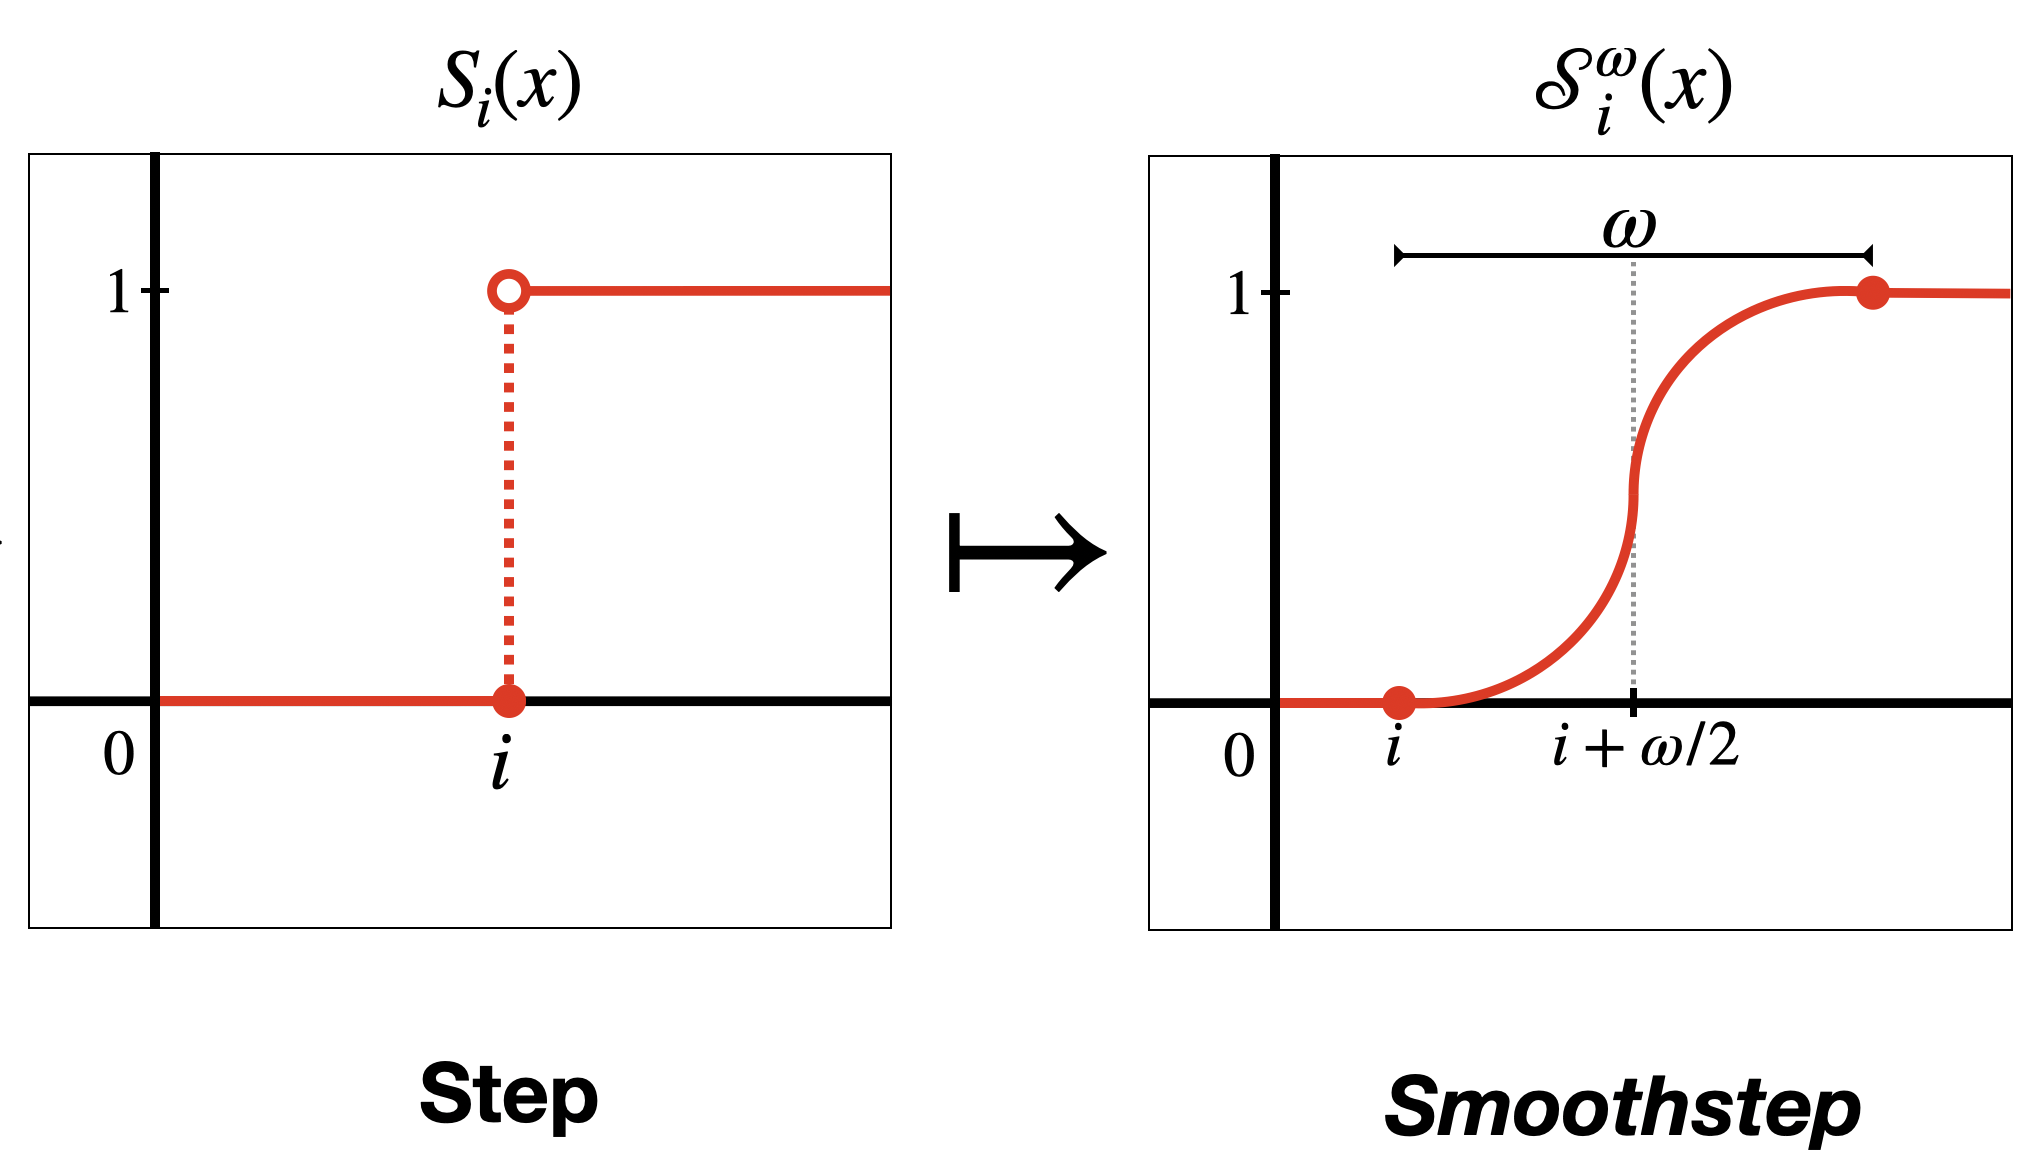
\includegraphics[width=0.88\textwidth,height=1\textheight]{smoothstep.png}

}

\end{figure}

Replacing \(S \mapsto \mathcal{S}\) ensures \(\partial_p^{i,j}(\alpha)\)
is element-wise continuous

\textbf{Note}: \(\partial_p^{i,j}(\alpha)\) has rank
\(= \mathrm{rank}(R_p^{i,j}(\alpha))\) for all
\(\alpha \in \mathbb{R}\).

\hypertarget{spectral-functions}{%
\subsection{Spectral functions}\label{spectral-functions}}

\textbf{Idea \#2}: Approximate \(\mathrm{rank}\) with \emph{spectral
functions} (Bhatia 2013)

\(\quad\quad\quad\quad \mathrm{rank}(X) = \lVert \mathbf{\sigma} \rVert_0\)

\(\quad\quad\quad\quad \hphantom{\mathrm{rank}(X)} = \sum\limits_{i=1}^{n} \, \mathrm{sgn}_+(\sigma_i)\)

\(\quad\quad\quad\quad \hphantom{\mathrm{rank}(X)}\approx \sum\limits_{i=1}^n \, \phi(\sigma_i, \epsilon)\)

\(\quad\quad\quad\quad \hphantom{\mathrm{rank}(X)}=\lVert \Phi_\epsilon(X) \rVert_\ast \vphantom{\sum\limits_{i=1}^n}\)

where \(\quad\quad\) \(X = U \mathrm{Diag}(\mathbf{\sigma})V^T\)

where \(\quad\quad\)
\(\mathrm{sgn}_{+}(x) \triangleq \mathbf{1}(x > 0)\vphantom{\sum\limits_{i=1}^n}\)

where \(\quad\quad\)
\(\phi(x, \epsilon) \triangleq \int\limits_{-\infty}^x\hat{\delta}(z, \epsilon) dz\vphantom{\sum\limits_{i=1}^n}\)

where \(\quad\quad\)
\(\Phi_\epsilon(X) \triangleq \sum_{i=1}^n \phi(\sigma_i, \epsilon) u_i v_i^T\)

\(\Phi_\epsilon(X)\) is a \emph{Löwner operator} when \(\phi\) is
\emph{operator monotone} (Jiang and Sendov 2018)

\[ A \succeq B \implies \Phi_\epsilon(A) \succeq \Phi_\epsilon(B) \]

Used in convex analysis + nonexpansive mappings (Bauschke, Combettes, et
al. 2011)

Spectral approximations to rank

\hypertarget{lowner-operators}{%
\subsection{Lowner Operators}\label{lowner-operators}}

(Bi, Han, and Pan 2013) show that for any smoothed Dirac delta
function\footnote{Any \(\hat{\delta}\) of the form
  \(\nu(1/\epsilon) p (z \cdot \nu (1/\epsilon))\) where \(p\) is a
  density function and \(\nu\) positive and increasing is sufficient.}
\(\hat{\delta}\) and differentiable \emph{operator monotone} function
\(\phi: \mathbb{R}_+ \times \mathbb{R}_{++} \to \mathbb{R}_+\), we have:

(\(\epsilon\)-close)

(Monotonicity)

(Smooth)

(Computable)

(Differentiable)

\(0 \leq \mathrm{rank}(X) - \lVert \Phi_\epsilon(X) \rVert_\ast \leq c(\hat{\delta})\)

\(\lVert \Phi_{\epsilon}(X) \rVert_\ast \geq \lVert \Phi_{\epsilon'}(X) \rVert_\ast\)
for any \(\epsilon \leq \epsilon'\)

Lipshitz + semismooth\footnote{Here \emph{semismooth} refers the
  existence of directional derivatives} on \(\mathbb{R}^{n \times m}\)

Closed-form soln. to differential
\(\partial \lVert \Phi_\epsilon(\cdot) \rVert_\ast\)

Continuously differentiable on \(\mathbf{S}_+^m\)

Small issue:
\(\quad \partial_p^\ast(\alpha) \in \mathbb{R^{n \times m}}\) (not in
\(\mathbf{S}_+^m\))

Easy fix: \(\quad\)
\(\Phi_\epsilon(\partial_p \circ \partial_p^T)(\alpha)\) \(\quad\) or
\(\quad\) \(\Phi_\epsilon(\partial_p^T \circ \partial_p)(\alpha)\)

\hypertarget{combinatorial-laplacian}{%
\subsection{Combinatorial Laplacian}\label{combinatorial-laplacian}}

\textbf{3rd idea:} parameterize using \emph{combinatorial Laplacians}
(Horak and Jost 2013):

\[ \Delta_p = \underbrace{\partial_{p+1} \partial_{p+1}^T}_{L_p^{\mathrm{up}}}  + \underbrace{\partial_{p}^T \partial_{p}}_{L_p^{\mathrm{dn}}} \]

\(f_\alpha\) is 1-to-1 correspondence with inner products on cochain
groups \(C^p(K, \mathbb{R})\)

\[L_p^{i,j}(\alpha) \Leftrightarrow \langle \; f,\, g \; \rangle_{\alpha} \text{ on } C^{p+1}(K)\]

Have ``nice'' linear and quadratic forms, e.g.: \[
L_p^{\text{up}}(\tau, \tau')= \begin{cases}
         \mathrm{deg}_f(\tau) \cdot f^{+/2}(\tau) & \text{ if } \tau = \tau' \\ 
%       \mathrm{deg}(\tau_i) & \text{ if } i = j \\ 
        s_{\tau, \tau'} \cdot  f^{+/2}(\tau) \cdot f(\sigma) \cdot f^{+/2}(\tau') & \text{ if } \tau \overset{\sigma}{\sim} \tau' \\
        0 & \text{ otherwise} 
    \end{cases}
\]

\(\implies\) can represent operator in ``matrix-free'' fashion

\hypertarget{regularization-interpretation}{%
\subsection{Regularization
interpretation}\label{regularization-interpretation}}

Instead of solving \(Ax = b\), consider the ``regularized''
least-squares objective:

\[
x_\epsilon^\ast = \argmin\limits_{x \in \mathbb{R}^n} \lVert Ax - b\rVert^2 + \epsilon \lVert x \rVert_1 
\]

The minimizer is given in closed-form by the regularized pseudo-inverse:

\[
x_\epsilon^\ast = (A^T A + \epsilon I)^{-1} A^T b
\]

\begin{figure}

{\centering \includegraphics[width=0.5\textwidth,height=\textheight]{lasso.png}

}

\end{figure}

\hypertarget{regularization-interpretation-1}{%
\subsection{Regularization
interpretation}\label{regularization-interpretation-1}}

\[
x_\epsilon^\ast = \argmin\limits_{x \in \mathbb{R}^n} \lVert Ax - b\rVert^2 + \epsilon \lVert x \rVert^2 = (A^T A + \epsilon I)^{-1} A^T b
\]

Under the appropriate hyper-parameter settings\footnote{This \(\phi\)
  corresponds to setting \(\nu(\epsilon) = \sqrt{\epsilon}\) and
  \(p(x) = 2x (x^2 + 1)^{-2}\).}, \(\phi\) takes the form:

\[
\phi(x, \epsilon) = \int\limits_{-\infty}^x \hat{\delta}(z, \epsilon) dz = \frac{x^2}{x^2 + \epsilon}
\]

The corresponding Lowner operator and its Schatten \(1\)-norm is given
by:

\[
\Phi_\epsilon(X) = (X^T X + \epsilon \, I_n)^{-1} X^T X, \quad \quad \lVert \Phi_\epsilon(X) \rVert_\ast = \sum\limits_{i = 1}^n \frac{\sigma_i(X)^2}{\sigma_i(X)^2 + \epsilon}
\]

This the \emph{Tikhonov regularization} in standard form used in
\(\ell_1\)-regression (LASSO)

\hypertarget{summary-of-relaxation}{%
\subsection{Summary of relaxation}\label{summary-of-relaxation}}

\[
\begin{align*}
\mu_p^R(K_\bullet, f) &\triangleq \mathrm{card}\big(\, \left.\mathrm{dgm}(K, \, f_\alpha) \right|_{R} \, \big) \\
&= \mathrm{rank}(\partial_{p+1}^{j+1,k}) + \dots \\
\hat{\mu}_p^R(K, f_\alpha) &= \mathrm{rank}(\hat{\partial}_{p+1}^{j+1, k}(\alpha)) + \dots  \\
&\approx \lVert \Phi_{\epsilon}(\hat{\partial}_{p+1}^{j+1, k}(\alpha)) \rVert_\ast + \dots \\
&= \lVert \Phi_{\epsilon}(L_p^\ast(\alpha)) \rVert_\ast \\
& \Leftrightarrow \langle \; f,\, g \; \rangle_{\alpha} \text{ on } C^{p+1}(K)
\end{align*} 
\]

By construction, \(\hat{\mu}_p^R(K, f_\alpha)\) is not only continuous,
but varying \(\alpha \in \mathbb{R}\) traces out a curve in
\(\mathbf{S}_+\)

\hypertarget{overview-1}{%
\subsection{Overview}\label{overview-1}}

\begin{itemize}
\tightlist
\item
  Introduction \& Motivation

  \begin{itemize}
  \tightlist
  \item
    Diagram vectorization and optimization
  \item
    The effective intractability of reduction
  \item
    Duality between diagrams and their ranks
  \end{itemize}
\end{itemize}

\begin{itemize}
\tightlist
\item
  Derivation of relaxation

  \begin{itemize}
  \tightlist
  \item
    Parameterizing \(p\)-chains with \(\mathbb{R}\) coefficients
  \item
    Replacing boundary operators with Löwner operators
  \item
    Connections to combinational Laplacians
  \end{itemize}
\end{itemize}

\begin{itemize}
\tightlist
\item
  Experiments

  \begin{itemize}
  \tightlist
  \item
    Shape signatures via directional transform
  \item
    Shape signatures via intrinsic metrics\\
  \item
    Codensity example
  \end{itemize}
\end{itemize}

\hypertarget{experiment-1-directional-transform}{%
\subsection{Experiment \#1: Directional
Transform}\label{experiment-1-directional-transform}}

Consider ``looking'' at a complex \(K\) embedded in \(R^d\)

\[\begin{align*}
\mathrm{DT}(K): S^{d-1} &\to  K \times C(K, \mathbb{R}) \\
    v &\mapsto (K_\bullet, f_v)
\end{align*}
\]

\begin{figure}

{\centering \includegraphics[width=4.16667in,height=1\textheight]{dt.png}

}

\end{figure}

\[
K_\bullet = K(v)_i = \{\, x \in X \mid \langle x, v \rangle \leq i  \,\}
\]

\hypertarget{experiment-1-directional-transform-1}{%
\subsection{Experiment \#1: Directional
Transform}\label{experiment-1-directional-transform-1}}

\[
K_\bullet = K(v)_i = \{\, x \in X \mid \langle x, v \rangle \leq i  \,\}
\]

\begin{figure}

{\centering \includegraphics[width=4.16667in,height=1\textheight]{dt.png}

}

\end{figure}

\[\{ \; \mathrm{dgm}(v) : v \in S^{d-1} \; \} \Leftrightarrow \mathrm{PHT} \]

\[\{ \; \chi(v) : v \in S^{d-1} \; \} \Leftrightarrow \mathrm{ECT} \]

\hypertarget{experiment-1-directional-transform-2}{%
\subsection{Experiment \#1: Directional
Transform}\label{experiment-1-directional-transform-2}}

\[
K_\bullet = K(v)_i = \{\, x \in X \mid \langle x, v \rangle \leq i  \,\}
\]

Injectivity of the PHT \(\leftrightarrow\) endow a metric
\(\mathcal{D}\) by integrating \(d_B\) (or \(d_W\)) over \(S_{d-1}\)

\[ \operatorname{d}_{\mathrm{PHT}}\left(\mathrm{dgm}_X, \mathrm{dgm}_Y\right):=\sum_{p=0}^d \int_{S^{d-1}} \operatorname{d}_B\left(\mathrm{dgm}(X, v) \right), \left( \mathrm{dgm}(X, v) \right) dv \]

\begin{figure}

\begin{minipage}[t]{0.50\linewidth}

{\centering 

\raisebox{-\height}{

\includegraphics[width=6.77083in,height=\textheight]{turtle1.png}

}

}

\end{minipage}%
%
\begin{minipage}[t]{0.50\linewidth}

{\centering 

\raisebox{-\height}{

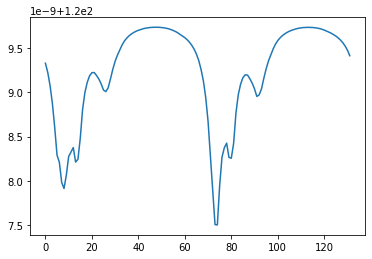
\includegraphics[width=6.77083in,height=\textheight]{turtle2.png}

}

}

\end{minipage}%

\end{figure}

\hypertarget{experiment-1-directional-transform-3}{%
\subsection{Experiment \#1: Directional
Transform}\label{experiment-1-directional-transform-3}}

\[
K_\bullet = K(v)_i = \{\, x \in X \mid \langle x, v \rangle \leq i  \,\}
\]

Injectivity of the PHT \(\leftrightarrow\) endow a metric
\(\mathcal{D}\) by integrating \(d_B\) (or \(d_W\)) over \(S_{d-1}\)

\[ \operatorname{d}_{\mathrm{PHT}}\left(\mathrm{dgm}_X, \mathrm{dgm}_Y\right):=\sum_{p=0}^d \int_{S^{d-1}} \operatorname{d}_B\left(\mathrm{dgm}(X, v) \right), \left( \mathrm{dgm}(X, v) \right) dv \]

\begin{figure}

\begin{minipage}[t]{0.50\linewidth}

{\centering 

\raisebox{-\height}{

\includegraphics[width=6.77083in,height=\textheight]{turtle1.png}

}

}

\end{minipage}%
%
\begin{minipage}[t]{0.50\linewidth}

{\centering 

\raisebox{-\height}{

\includegraphics[width=6.77083in,height=\textheight]{bone1.png}

}

}

\end{minipage}%

\end{figure}

\hypertarget{experiment-1-directional-transform-4}{%
\subsection{Experiment \#1: Directional
Transform}\label{experiment-1-directional-transform-4}}

\begin{figure}

{\centering 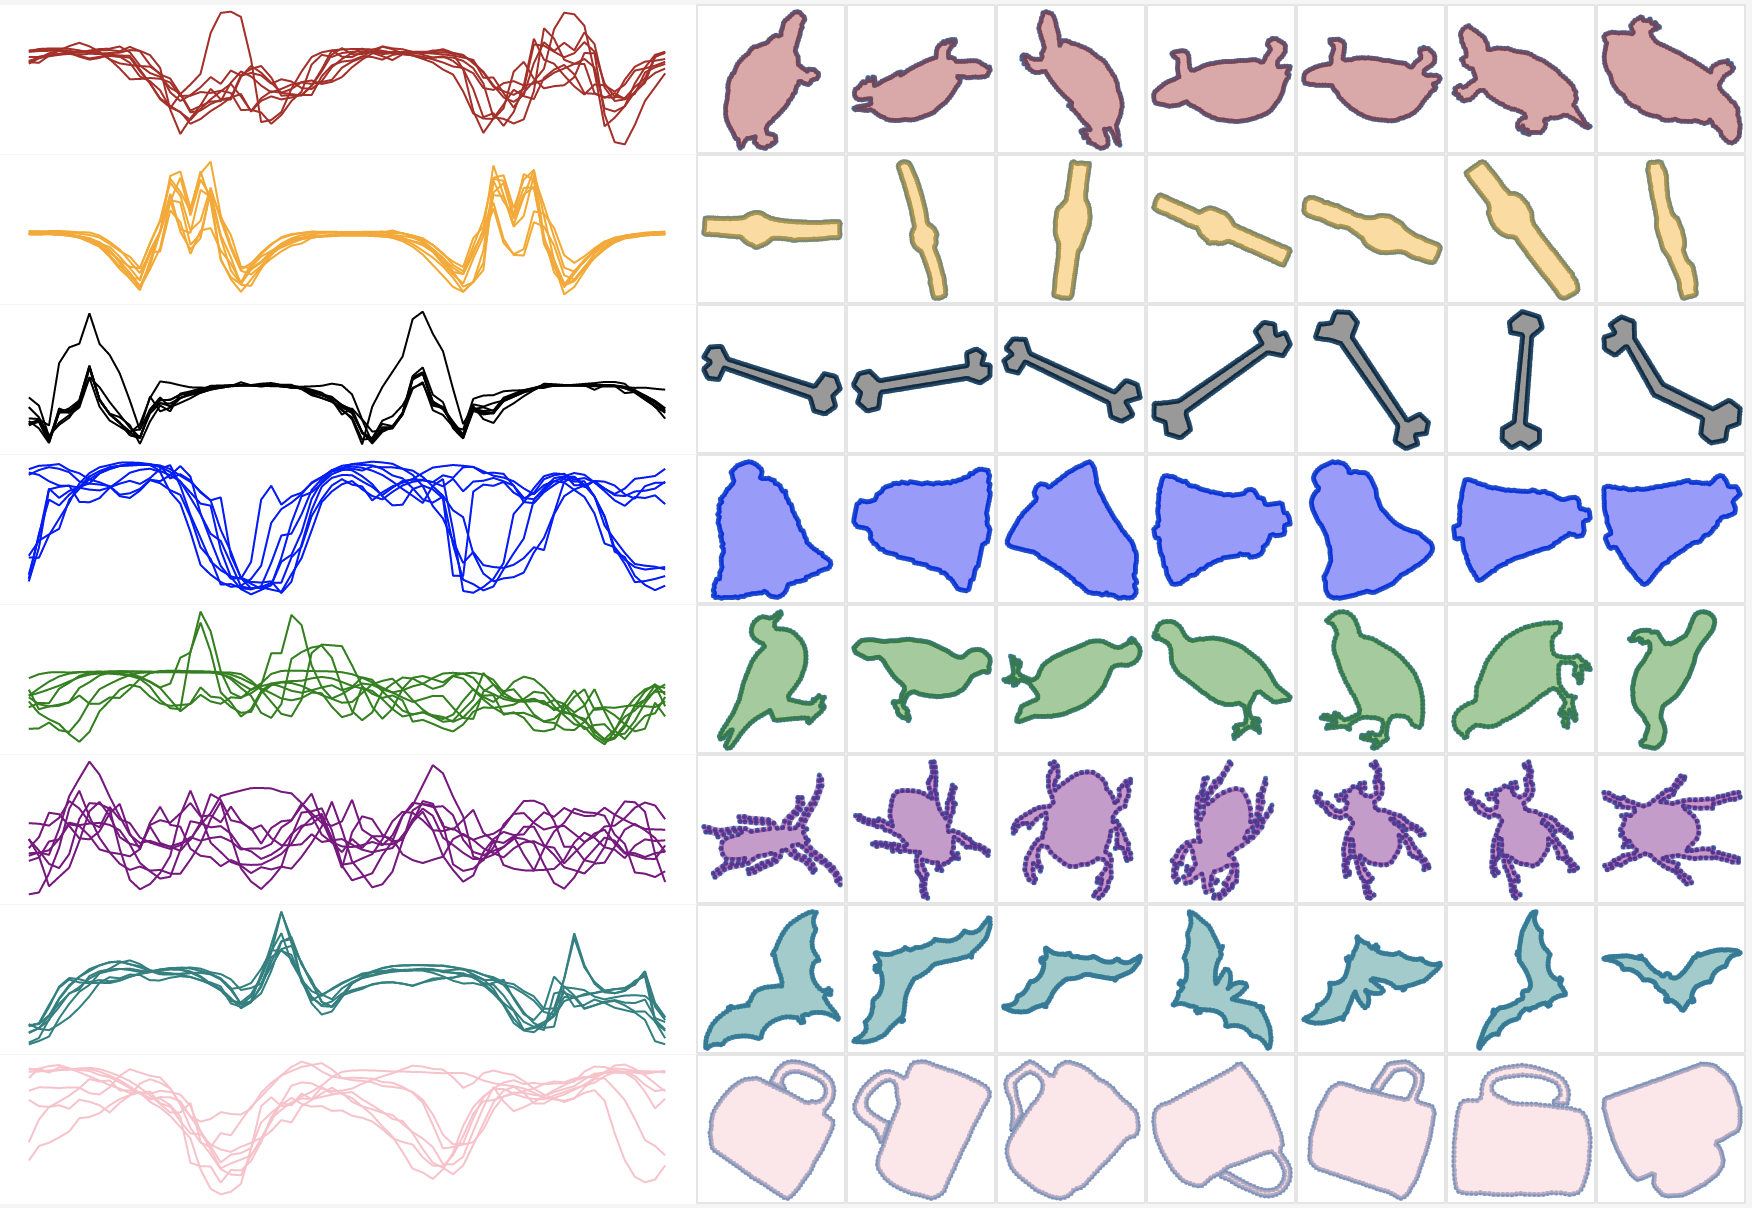
\includegraphics[width=0.8\textwidth,height=1\textheight]{shape_signatures.png}

}

\end{figure}

Luis mentioned modding out rotations and translations adn scale to
compare shapes. We can handle rotations via phase alignment.

Sarah mentioned handling orientation.

\hypertarget{experiment-2-intrinsic-signatures}{%
\subsection{Experiment \#2: Intrinsic
signatures}\label{experiment-2-intrinsic-signatures}}

\textbf{Dataset:} 3D meshes of animals in different poses (Chazal et al.
2009)

\begin{figure}

{\centering \includegraphics[width=4.42708in,height=1\textheight]{gh_data_pose.png}

}

\end{figure}

\textbf{Challenge:} Recognize intrinsic shape categories (via a distance
metric)

\hypertarget{experiment-2-intrinsic-signatures-1}{%
\subsection{Experiment \#2: Intrinsic
signatures}\label{experiment-2-intrinsic-signatures-1}}

The \emph{Gromov-Hausdorff} distance yields a metric on the set of
compact metric spaces \(\mathcal{X}\)

\[
d_{GH}(d_X, d_Y) = \sup_{x \in X, y \in Y} \lvert d_X(x, \psi(y)) - d_Y(y, \phi(x))\rvert 
\]

\begin{figure}

{\centering \includegraphics[width=6.25in,height=1\textheight]{camel_gh.png}

}

\end{figure}

Using intrinsic metric makes \(d_{\mathrm{GH}}\) blind to e.g.~shapes
represented in different \emph{poses}

Unfortunately, the GH distance is NP-hard to compute (Mémoli 2012)

\hypertarget{experiment-2-intrinsic-signatures-2}{%
\subsection{Experiment \#2: Intrinsic
signatures}\label{experiment-2-intrinsic-signatures-2}}

It's known \(d_B\) (\(d_W\)) on Rips filtrations \(\mathcal{R}(X, d_X)\)
lower bound GH (GW) distance

\[ 
d_B(\mathrm{dgm}_p(\mathcal{R}(X, d_X)), \mathrm{dgm}_p(\mathcal{R}(Y, d_Y))) \; \leq \; d_{GH}((X, d_X), (Y, d_Y))
\]

\begin{figure}

\begin{minipage}[t]{\linewidth}

{\centering 

\raisebox{-\height}{

\includegraphics[width=9.11458in,height=\textheight]{camel_gh_rips_comparison.png}

}

}

\end{minipage}%

\end{figure}

Motivates use of persistence in metric settings for e.g.~shape
classification!

\hypertarget{experiment-2-intrinsic-signatures-3}{%
\subsection{Experiment \#2: Intrinsic
signatures}\label{experiment-2-intrinsic-signatures-3}}

\textbf{Issue:} Diagrams are far from injective, cannot distinguish
e.g.~stretched shapes

\begin{figure}

{\centering \includegraphics[width=5.98958in,height=1\textheight]{dgm_noninjective.png}

}

\end{figure}

The lower bound on \(d_{\mathrm{GH}}\) could be totally useless!

\hypertarget{experiment-2-intrinsic-signatures-4}{%
\subsection{Experiment \#2: Intrinsic
signatures}\label{experiment-2-intrinsic-signatures-4}}

Lower bounds extend to Rips filtrations \emph{augmented} with
real-valued functions \(f, g\):

\[
\mathcal{R}(f) \triangleq \mathcal{R}(X, d_X, f) = \{\mathcal{R}_\alpha(X_\alpha)\}_{\alpha > 0}, \quad X_\alpha \triangleq f^{-1}((-\infty, \alpha)) \subseteq X
\]

The diagrams from \(\mathcal{R}(\lambda \cdot f_X)\) represent
\emph{stable signatures} for each \(\lambda > 0\):

\[
d_B(\mathcal{R}(\lambda \cdot f_X), \mathcal{R}(\lambda \cdot f_Y)) \leq \max(1, \lambda L) \cdot d_{\mathrm{GH}}(X, Y)
\]

Chazal showed these bounds extend to metrics on \emph{augmented} metric
spaces:

\[
\mathcal{X}_1 = \{ (X, d_X, f_X) \mid (X, d_X, f_X) \in \mathcal{X}, f_X: X \to \mathbb{R} \text{ continuous }\}
\]

These signatures also extend to measure metric spaces, see (Chazal et
al. 2009)

{ NOTE: } Size of \(L\) depends on the choice of \(f\) + each
\(\lambda\) produces a new signature!

\hypertarget{experiment-2-intrinsic-signatures-5}{%
\subsection{Experiment \#2: Intrinsic
signatures}\label{experiment-2-intrinsic-signatures-5}}

\textbf{Ex:} The \emph{eccentricity} function
\(e_X^1(x) = \max_{x' \in X} d_X(x,x')\) has \(L = 2\)

\begin{figure}

{\centering \includegraphics[width=8.07292in,height=1\textheight]{dgm_noninjective2.png}

}

\end{figure}

Augmenting via a fraction of \(e_X^1\) modifies the diagrams of the
ellipsoid significantly

\hypertarget{experiment-2-intrinsic-signatures-6}{%
\subsection{Experiment \#2: Intrinsic
signatures}\label{experiment-2-intrinsic-signatures-6}}

Lower bounds extend to Rips filtrations \emph{augmented} with
real-valued functions \(f, g\):

\[
d_B(\mathcal{R}(\lambda \cdot f_X), \mathcal{R}(\lambda \cdot f_Y)) \leq \max(1, \lambda L) \cdot d_{\mathrm{GH}}(X, Y)
\]

\begin{figure}

\begin{minipage}[t]{0.25\linewidth}

{\centering 

\raisebox{-\height}{

\includegraphics[width=4.6875in,height=\textheight]{camel1_rips.png}

}

}

\end{minipage}%
%
\begin{minipage}[t]{0.25\linewidth}

{\centering 

\raisebox{-\height}{

\includegraphics[width=4.6875in,height=\textheight]{camel_dgm_rips.png}

}

}

\end{minipage}%
%
\begin{minipage}[t]{0.25\linewidth}

{\centering 

\raisebox{-\height}{

\includegraphics[width=4.6875in,height=\textheight]{camel1_ecc.png}

}

}

\end{minipage}%
%
\begin{minipage}[t]{0.25\linewidth}

{\centering 

\raisebox{-\height}{

\includegraphics[width=4.6875in,height=\textheight]{camel_dgm_ecc.png}

}

}

\end{minipage}%

\end{figure}

Larger values of \(\lambda\) yield worse bounds, but can lead to simpler
diagrams

\hypertarget{experiment-2-intrinsic-signatures-7}{%
\subsection{Experiment \#2: Intrinsic
signatures}\label{experiment-2-intrinsic-signatures-7}}

Each choice of \(\lambda > 0\) yields a \emph{stable signature} via
\(\mathcal{R}(\lambda \cdot f_X)\)

Which value of \(\lambda\) to choose?

\begin{figure}

{\centering \includegraphics[width=9.89583in,height=1\textheight]{camel1_interp1.png}

}

\end{figure}

\hypertarget{experiment-2-intrinsic-signatures-8}{%
\subsection{Experiment \#2: Intrinsic
signatures}\label{experiment-2-intrinsic-signatures-8}}

Each choice of \(\lambda > 0\) yields a \emph{stable signature} via
\(\mathcal{R}(\lambda \cdot f_X)\)

Which value of \(\lambda\) to choose?

\begin{figure}

{\centering \includegraphics[width=9.89583in,height=1\textheight]{camel1_interp2.png}

}

\end{figure}

We sample from \(\Delta_+\) randomly, retaining signatures with
sufficient topological activity

\hypertarget{experiment-2-intrinsic-signatures-9}{%
\subsection{Experiment \#2: Intrinsic
signatures}\label{experiment-2-intrinsic-signatures-9}}

\ldots and compared the computed spectral signatures under the relative
distance metric:

\[
\Lambda(\mu_p^R) = \{\sigma_1, \sigma_2, \dots, \sigma_n \}, \quad \quad \chi(\mathbf{\sigma}, \mathbf{\tilde{\sigma}}) = \sum\limits_{i=1}^n \frac{\lvert \sigma_i - \tilde{\sigma}_i \rvert}{\sqrt{\sigma_i + \tilde{\sigma}_i}}
\]

\begin{figure}

{\centering \includegraphics[width=7.8125in,height=1\textheight]{dw_chi_comp.png}

}

\end{figure}

\hypertarget{experiment-3-filtration-optimization}{%
\subsection{Experiment \#3: Filtration
optimization}\label{experiment-3-filtration-optimization}}

\begin{figure}

\begin{minipage}[b]{0.25\linewidth}

{\centering 

\includegraphics{vineyard.gif}

}

\end{minipage}%
%
\begin{minipage}[b]{0.50\linewidth}

{\centering 

\includegraphics{dgm_opt.png}

}

\end{minipage}%
%
\begin{minipage}[b]{0.25\linewidth}

{\centering 

\includegraphics{complex_plain.gif}

}

\end{minipage}%

\end{figure}

\[ 
\alpha^\ast = \argmax_{\alpha \in \mathbb{R}} \; \mathrm{card}\big(\, \left.\mathrm{dgm}(K_\bullet, \, f_\alpha) \right|_{R} \, \big) 
\]

\hypertarget{experiment-3-filtration-optimization-1}{%
\subsection{Experiment \#3: Filtration
optimization}\label{experiment-3-filtration-optimization-1}}

\begin{figure}

\begin{minipage}[b]{0.67\linewidth}

{\centering 

\includegraphics{codensity_mult.png}

}

\end{minipage}%
%
\begin{minipage}[b]{0.33\linewidth}

{\centering 

\includegraphics{optimal_codensity_complex.png}

}

\end{minipage}%

\end{figure}

\[ 
\alpha^\ast = \argmax_{\alpha \in \mathbb{R}} \; \mathrm{card}\big(\, \left.\mathrm{dgm}(K_\bullet, \, f_\alpha) \right|_{R} \, \big) 
\]

\hypertarget{experiment-3-filtration-optimization-2}{%
\subsection{Experiment \#3: Filtration
optimization}\label{experiment-3-filtration-optimization-2}}

\begin{figure}

{\centering \includegraphics{codensity_ex1.png}

}

\end{figure}

\[
\mathrm{rank}(X) = \sum\limits_{i=1}^{n} \, \mathrm{sgn}_+(\sigma_i)
\]

\[ 
\mu_p^{R} = \mathrm{rank}(\partial_{p+1}^{j + 1, k})  - \mathrm{rank}(\partial_{p+1}^{i + 1, k})  - \mathrm{rank}(\partial_{p+1}^{j + 1, l}) + \mathrm{rank}(\partial_{p+1}^{i + 1, l})  
\]

\hypertarget{experiment-3-filtration-optimization-3}{%
\subsection{Experiment \#3: Filtration
optimization}\label{experiment-3-filtration-optimization-3}}

\begin{figure}

{\centering \includegraphics{codensity_ex2.png}

}

\end{figure}

\[
\lVert X \rVert_\ast = \sum\limits_{i=1}^{n} \, \lvert \sigma_i \rvert 
\]

\[ 
\hat{\mu}_p^{R} = \lVert \partial_{p+1}^{j + 1, k}\rVert_\ast  -  \lVert \partial_{p+1}^{i + 1, k}\rVert_\ast  -  \lVert \partial_{p+1}^{j + 1, l}\rVert_\ast +  \lVert \partial_{p+1}^{i + 1, l} \rVert_\ast
\]

\hypertarget{experiment-3-filtration-optimization-4}{%
\subsection{Experiment \#3: Filtration
optimization}\label{experiment-3-filtration-optimization-4}}

\begin{figure}

{\centering \includegraphics{codensity_ex3.png}

}

\end{figure}

\[
\lVert \Phi_\epsilon(X) \rVert_\ast = \sum\limits_{i=1}^{n} \, \phi(\lvert \sigma_i \rvert, \epsilon), \quad \quad \epsilon = 0.30
\]

\hypertarget{experiment-3-filtration-optimization-5}{%
\subsection{Experiment \#3: Filtration
optimization}\label{experiment-3-filtration-optimization-5}}

\includegraphics{combinatorial_explosion.png}\footnote{Xu, Weiyu, and
  Babak Hassibi. ``Precise Stability Phase Transitions for \$\ell\_1 \$
  Minimization: A Unified Geometric Framework.'' IEEE transactions on
  information theory (2011)}

\hypertarget{experiment-3-filtration-optimization-6}{%
\subsection{Experiment \#3: Filtration
optimization}\label{experiment-3-filtration-optimization-6}}

\begin{figure}

{\centering \includegraphics{codensity_ex4.png}

}

\end{figure}

\[
\lVert \Phi_\epsilon(X) \rVert_\ast = \sum\limits_{i=1}^{n} \, \phi(\lvert \sigma_i \rvert, \epsilon), \quad \quad \epsilon = 0.10
\]

\hypertarget{experiment-3-filtration-optimization-7}{%
\subsection{Experiment \#3: Filtration
optimization}\label{experiment-3-filtration-optimization-7}}

\begin{figure}

{\centering \includegraphics{codensity_ex5.png}

}

\end{figure}

\[
\lVert \Phi_\epsilon(X) \rVert_\ast = \sum\limits_{i=1}^{n} \, \phi(\lvert \sigma_i \rvert, \epsilon), \quad \quad \epsilon \to 0^+
\]

\hypertarget{time-permitting-computation}{%
\subsection{Time permitting:
Computation}\label{time-permitting-computation}}

Spectra of Laplacian operators well-studied:

\begin{itemize}
\tightlist
\item
  Iterative Krylov methods / Lanczos dominate solving sparse
  systems\(^2\)
\item
  Many laplacian preconditioning methods known (Jambulapati and Sidford
  2021)
\item
  Nearly optimal algorithms known for SDD (Stathopoulos and McCombs
  2007)
\end{itemize}

\textbf{Theorem (Simon 1984)}: Given a symmetric rank-\(r\) matrix
\(A \in \mathbb{R}^{n \times n}\) whose matrix-vector operator
\(A \mapsto A x\) requires \(O(\eta)\) time and \(O(\nu)\) space, the
Lanczos iteration computes
\(\Lambda(A) = \{ \lambda_1, \lambda_2, \dots, \lambda_r \}\) in
\(O(\max\{\eta, n\}\cdot r)\) time and \(O(\max\{\nu, n\})\) space done
in exact arithmetic.

\begin{itemize}
\tightlist
\item
  Permutation invariance \(\implies\) can optimize memory access of
  \(\mathtt{SpMat}\) operation
\end{itemize}

\begin{itemize}
\tightlist
\item
  Any complex data structure suffices, e.g.~tries\(^2\), combinadics,
  etc\ldots{}
\end{itemize}

\marginnote{\begin{footnotesize}

See Parlett (1995) for an overview of the Lanczos. See (Boissonnat and
Maria 2014) for representing complexes.

\end{footnotesize}}

\hypertarget{time-permitting-computation-1}{%
\subsection{Time permitting:
Computation}\label{time-permitting-computation-1}}

Preliminary experiments suggest the scalability is promising

\includegraphics{watts_strogatz_perf.png}

\begin{itemize}
\tightlist
\item
  \(\approx \, \leq 25\) Lanczos vectors to approximate full spectrum at
  \(\epsilon > 0\)
\item
  \(\implies O(n)\) memory to obtain \(\lVert \cdot \rVert_\ast\) in
  \(O(n^2)\) time (with small constants!)
\item
  Larger values \(\epsilon\) or lower numerical tolerances \(\implies\)
  essentially linear time compute
\item
  Previousy computed eigenvectors can be re-used for ``warm restarts''
\end{itemize}

\hypertarget{conclusion}{%
\subsection{Conclusion}\label{conclusion}}

Spectral relaxation of rank invariant using Löwner operators

\begin{itemize}
\tightlist
\item
  Suitable for parameterized families of filtrations
\item
  Differentiable + amenable for optimization
\item
  Stable to perturbations in \(f_\alpha\) when \(\epsilon > 0\), but
  unstable as as \(\epsilon \to 0^+\)
\item
  Excellent compute properties. Implementation ongoing.
\item
  Better optimizer implementation also ongoing.
\end{itemize}

Looking for collaborators! In particular:

\begin{itemize}
\tightlist
\item
  Optimizing parameterized filtrations
\item
  Differentiating n-parameter families of filtrations
\item
  Encoding features with Laplacian spectra
\item
  Sparse minimization problems (compressive sensing)
\item
  Understanding connections to other areas of math
\end{itemize}

\hypertarget{references}{%
\subsection{References}\label{references}}

\hypertarget{refs}{}
\begin{CSLReferences}{1}{0}
\leavevmode\vadjust pre{\hypertarget{ref-adams2017persistence}{}}%
Adams, Henry, Tegan Emerson, Michael Kirby, Rachel Neville, Chris
Peterson, Patrick Shipman, Sofya Chepushtanova, Eric Hanson, Francis
Motta, and Lori Ziegelmeier. 2017. {``Persistence Images: A Stable
Vector Representation of Persistent Homology.''} \emph{Journal of
Machine Learning Research} 18.

\leavevmode\vadjust pre{\hypertarget{ref-anderson1969series}{}}%
Anderson Jr, William N, and Richard James Duffin. 1969. {``Series and
Parallel Addition of Matrices.''} \emph{Journal of Mathematical Analysis
and Applications} 26 (3): 576--94.

\leavevmode\vadjust pre{\hypertarget{ref-bauer2022keeping}{}}%
Bauer, Ulrich, Talha Bin Masood, Barbara Giunti, Guillaume Houry,
Michael Kerber, and Abhishek Rathod. 2022. {``Keeping It Sparse:
Computing Persistent Homology Revised.''} \emph{arXiv Preprint
arXiv:2211.09075}.

\leavevmode\vadjust pre{\hypertarget{ref-bauschke2011convex}{}}%
Bauschke, Heinz H, Patrick L Combettes, et al. 2011. \emph{Convex
Analysis and Monotone Operator Theory in Hilbert Spaces}. Vol. 408.
Springer.

\leavevmode\vadjust pre{\hypertarget{ref-ben1967geometry}{}}%
Ben-Israel, Adi. 1967. {``On the Geometry of Subspaces in Euclidean
n-Spaces.''} \emph{SIAM Journal on Applied Mathematics} 15 (5):
1184--98.

\leavevmode\vadjust pre{\hypertarget{ref-ben2015projectors}{}}%
---------. 2015. {``Projectors on Intersection of Subspaces.''}
\emph{Contemporary Mathematics} 636: 41--50.

\leavevmode\vadjust pre{\hypertarget{ref-bhatia2013matrix}{}}%
Bhatia, Rajendra. 2013. \emph{Matrix Analysis}. Vol. 169. Springer
Science \& Business Media.

\leavevmode\vadjust pre{\hypertarget{ref-bi2013approximation}{}}%
Bi, Shujun, Le Han, and Shaohua Pan. 2013. {``Approximation of Rank
Function and Its Application to the Nearest Low-Rank Correlation
Matrix.''} \emph{Journal of Global Optimization} 57 (4): 1113--37.

\leavevmode\vadjust pre{\hypertarget{ref-boissonnat2014simplex}{}}%
Boissonnat, Jean-Daniel, and Clément Maria. 2014. {``The Simplex Tree:
An Efficient Data Structure for General Simplicial Complexes.''}
\emph{Algorithmica} 70: 406--27.

\leavevmode\vadjust pre{\hypertarget{ref-bubenik2020persistence}{}}%
Bubenik, Peter. 2020. {``The Persistence Landscape and Some of Its
Properties.''} In \emph{Topological Data Analysis: The Abel Symposium
2018}, 97--117. Springer.

\leavevmode\vadjust pre{\hypertarget{ref-cerri2013betti}{}}%
Cerri, Andrea, Barbara Di Fabio, Massimo Ferri, Patrizio Frosini, and
Claudia Landi. 2013. {``Betti Numbers in Multidimensional Persistent
Homology Are Stable Functions.''} \emph{Mathematical Methods in the
Applied Sciences} 36 (12): 1543--57.

\leavevmode\vadjust pre{\hypertarget{ref-chazal2009gromov}{}}%
Chazal, Frédéric, David Cohen-Steiner, Leonidas J Guibas, Facundo
Mémoli, and Steve Y Oudot. 2009. {``Gromov-Hausdorff Stable Signatures
for Shapes Using Persistence.''} In \emph{Computer Graphics Forum},
28:1393--403. 5. Wiley Online Library.

\leavevmode\vadjust pre{\hypertarget{ref-chazal2016structure}{}}%
Chazal, Frédéric, Vin De Silva, Marc Glisse, and Steve Oudot. 2016.
\emph{The Structure and Stability of Persistence Modules}. Vol. 10.
Springer.

\leavevmode\vadjust pre{\hypertarget{ref-chen2011output}{}}%
Chen, Chao, and Michael Kerber. 2011. {``An Output-Sensitive Algorithm
for Persistent Homology.''} In \emph{Proceedings of the Twenty-Seventh
Annual Symposium on Computational Geometry}, 207--16.

\leavevmode\vadjust pre{\hypertarget{ref-dey2021computing}{}}%
Dey, Tamal K, Woojin Kim, and Facundo Mémoli. 2021. {``Computing
Generalized Rank Invariant for 2-Parameter Persistence Modules via
Zigzag Persistence and Its Applications.''} \emph{arXiv Preprint
arXiv:2111.15058}.

\leavevmode\vadjust pre{\hypertarget{ref-dey2022computational}{}}%
Dey, Tamal Krishna, and Yusu Wang. 2022. \emph{Computational Topology
for Data Analysis}. Cambridge University Press.

\leavevmode\vadjust pre{\hypertarget{ref-edelsbrunner2000topological}{}}%
Edelsbrunner, Herbert, David Letscher, and Afra Zomorodian. 2000.
{``Topological Persistence and Simplification.''} In \emph{Proceedings
41st Annual Symposium on Foundations of Computer Science}, 454--63.
IEEE.

\leavevmode\vadjust pre{\hypertarget{ref-horak2013spectra}{}}%
Horak, Danijela, and Jürgen Jost. 2013. {``Spectra of Combinatorial
Laplace Operators on Simplicial Complexes.''} \emph{Advances in
Mathematics} 244: 303--36.

\leavevmode\vadjust pre{\hypertarget{ref-jambulapati2021ultrasparse}{}}%
Jambulapati, Arun, and Aaron Sidford. 2021. {``Ultrasparse
Ultrasparsifiers and Faster Laplacian System Solvers.''} In
\emph{Proceedings of the 2021 ACM-SIAM Symposium on Discrete Algorithms
(SODA)}, 540--59. SIAM.

\leavevmode\vadjust pre{\hypertarget{ref-jiang2018unified}{}}%
Jiang, Tianpei, and Hristo Sendov. 2018. {``A Unified Approach to
Operator Monotone Functions.''} \emph{Linear Algebra and Its
Applications} 541: 185--210.

\leavevmode\vadjust pre{\hypertarget{ref-kim2020pllay}{}}%
Kim, Kwangho, Jisu Kim, Manzil Zaheer, Joon Kim, Frédéric Chazal, and
Larry Wasserman. 2020. {``Pllay: Efficient Topological Layer Based on
Persistent Landscapes.''} \emph{Advances in Neural Information
Processing Systems} 33: 15965--77.

\leavevmode\vadjust pre{\hypertarget{ref-komzsik2003lanczos}{}}%
Komzsik, Louis. 2003. \emph{The Lanczos Method: Evolution and
Application}. SIAM.

\leavevmode\vadjust pre{\hypertarget{ref-mccleary2022edit}{}}%
McCleary, Alexander, and Amit Patel. 2022. {``Edit Distance and
Persistence Diagrams over Lattices.''} \emph{SIAM Journal on Applied
Algebra and Geometry} 6 (2): 134--55.

\leavevmode\vadjust pre{\hypertarget{ref-memoli2012some}{}}%
Mémoli, Facundo. 2012. {``Some Properties of Gromov--Hausdorff
Distances.''} \emph{Discrete \& Computational Geometry} 48: 416--40.

\leavevmode\vadjust pre{\hypertarget{ref-memoli2022persistent}{}}%
Mémoli, Facundo, Zhengchao Wan, and Yusu Wang. 2022. {``Persistent
Laplacians: Properties, Algorithms and Implications.''} \emph{SIAM
Journal on Mathematics of Data Science} 4 (2): 858--84.

\leavevmode\vadjust pre{\hypertarget{ref-parlett1995we}{}}%
Parlett, Beresford N. 1995. {``Do We Fully Understand the Symmetric
Lanczos Algorithm Yet?''} CALIFORNIA UNIV BERKELEY DEPT OF MATHEMATICS.

\leavevmode\vadjust pre{\hypertarget{ref-piekenbrock2021move}{}}%
Piekenbrock, Matthew, and Jose A Perea. 2021. {``Move Schedules: Fast
Persistence Computations in Coarse Dynamic Settings.''} \emph{arXiv
Preprint arXiv:2104.12285}.

\leavevmode\vadjust pre{\hypertarget{ref-simon1984analysis}{}}%
Simon, Horst D. 1984. {``Analysis of the Symmetric Lanczos Algorithm
with Reorthogonalization Methods.''} \emph{Linear Algebra and Its
Applications} 61: 101--31.

\leavevmode\vadjust pre{\hypertarget{ref-som2020pi}{}}%
Som, Anirudh, Hongjun Choi, Karthikeyan Natesan Ramamurthy, Matthew P
Buman, and Pavan Turaga. 2020. {``Pi-Net: A Deep Learning Approach to
Extract Topological Persistence Images.''} In \emph{Proceedings of the
IEEE/CVF Conference on Computer Vision and Pattern Recognition
Workshops}, 834--35.

\leavevmode\vadjust pre{\hypertarget{ref-stathopoulos2007nearly}{}}%
Stathopoulos, Andreas, and James R McCombs. 2007. {``Nearly Optimal
Preconditioned Methods for Hermitian Eigenproblems Under Limited Memory.
Part II: Seeking Many Eigenvalues.''} \emph{SIAM Journal on Scientific
Computing} 29 (5): 2162--88.

\leavevmode\vadjust pre{\hypertarget{ref-zomorodian2004computing}{}}%
Zomorodian, Afra, and Gunnar Carlsson. 2004. {``Computing Persistent
Homology.''} In \emph{Proceedings of the Twentieth Annual Symposium on
Computational Geometry}, 347--56.

\end{CSLReferences}

\hypertarget{permutation-invariance}{%
\subsection{Permutation Invariance}\label{permutation-invariance}}

Consider the setting where \(f_\alpha : \mathbb{R} \to \mathbb{R}^N\) is
an \(\alpha\)-parameterized filter function:

\[ \mu_p^R(\, f_\alpha \, ) = \{ \mu_p^R(K_\bullet^\alpha) : \alpha \in \mathbb{R} \}\]

Difficult to compute \(R_\alpha = \partial_\alpha V_\alpha\) for all
\(\alpha\) as \(K_\bullet = (K, f_\alpha)\) is changing
constantly\ldots{}

\[ \mathrm{rank}(\partial_p(K_\bullet)) \equiv \mathrm{rank}(P^T \partial_p(K) P) \]
\[ \mathrm{rank}(\partial_p(K_\bullet)) \equiv \mathrm{rank}(W \mathrm{sgn}(\partial_p(K)) W) \]

Thus we may decouple \(f_\alpha\) and \(K\) in the computation:

\[
\begin{align*}
 \mu_p^{R}(K,f_\alpha) &\triangleq \mathrm{rank}\big(\,\hat{\partial}_{q}^{j + \delta, k}\,\big) - \; \dots \; + \mathrm{rank}\big(\, \hat{\partial}_{q}^{i + \delta, l}\,\big)  \\
&\equiv \mathrm{rank}\big(\,V_p^j \circ \partial_{q} \circ W_q^k \,\big) - \; \dots \; + \mathrm{rank}\big(\,V_p^{i+\delta} \circ \partial_{q} \circ W_q^l \,\big)
 \end{align*}
 \]

where the entries of \(V\), \(W\) change continuously w/ \(\alpha\),
while \(\partial_q\) remains \emph{fixed}\ldots{}

\hypertarget{spectral-functions-1}{%
\subsection{Spectral functions}\label{spectral-functions-1}}

Nuclear norm \(\lVert X \rVert_\ast = \lVert \mathbf{\sigma} \rVert_1\)
often used in sparse minimization problems like \emph{compressive
sensing} due to its convexity in the unit-ball
\(\{A \in \mathbb{R}^{n \times m} : \lVert A \rVert_2 \leq 1 \}\)

\begin{figure}

\begin{minipage}[b]{0.50\linewidth}

{\centering 

\includegraphics[width=3.125in,height=\textheight]{l0_l1.png}

}

\end{minipage}%
%
\begin{minipage}[b]{0.50\linewidth}

{\centering 

\includegraphics[width=3.33333in,height=\textheight]{convex_envelope.png}

}

\end{minipage}%

\end{figure}

\textbf{Left:} The \(\ell_0\) and \(\ell_1\) norms on the interval
\([-1,1]\)

\textbf{Right:} \(g\) forms the convex envelope of \(f\) in the interval
\([a,b]\)

\hypertarget{spectral-functions-2}{%
\subsection{Spectral functions}\label{spectral-functions-2}}

Unfortunately, \(\lVert \cdot \rVert_\ast\) often a poor substitute for
rank

\begin{figure}

{\centering \includegraphics[width=0.7\textwidth,height=1\textheight]{rank_relax.png}

}

\end{figure}

\textbf{Left:} The \(\ell_0\) and \(\ell_1\) norms on the interval
\([-1,1]\) \textbf{Right:}



\end{document}
